\chapter{Background Review}
In this chapter, we first briefly review spectral analysis in the context of 
shape analysis, including the theories and applications of Laplacian 
eigenstructures and spectral graph wavelets. Then we give an overview of the 
concept of sparse representation modeling as well as its related computational 
methods and applications in signal processing.

\section{Laplacian and Graph Fourier Transform}

\subsection*{Laplacian and Spectral Transform}
Fourier transform is perhaps the most fundamental tool for classical 
time-frequency (or space-frequency) signal analysis. The key idea is to decompose 
a temporal/spatial signal into the linear combinations of a set of sinusoid 
functions (i.e., the Fourier basis) of different frequencies. The collection of 
Fourier basis functions $\{\phi_n;n\in \mathbb{Z}\}$ form a complete orthogonal 
basis~\cite{Gomes:1999} of the underlying function space $\mathcal{F}$, and the 
transform coefficients gives a frequency-domain representation of the original
signal. In generally, this decomposition can be written as

\begin{equation}
f=\sum_{k=-\infty}^\infty \langle f,\phi_k\rangle\phi_k
\end{equation}

We first consider the classical Fourier analysis in $\mathbb{R}^1$. From the 
perspective of differential equations, the $k$th Fourier basis function 
$\phi_k(x)$ satisfies the following Helmholtz equation in $\mathbb{R}^1$

\begin{equation}\label{eq:Helmholtz1D}
-\frac{\partial^2 \phi_k(x)}{\partial x^2}=\omega_k^2 \phi_k(x).
\end{equation}

This is to say, in 1D Euclidean space, the Fourier basis functions are actually 
the eigenfunctions of the second order differential operator (i.e. Laplace operator)
$\frac{\partial^2}{\partial x^2}$.

The concept of Fourier transform can be generalized to the manifold domain.
Given a manifold $\mathcal{M}$ with Riemannian metric $g$. The goal is to find a
family of functions $\{\phi_k(x)\}$ that form a orthonormal and complete
basis of the Hilbert space $\L^2(\mathcal{M,g}):\mathcal{M}\to\mathbb{R}$ with
properties similar to the classical Fourier basis. In manifold space, the equivalent
to the Laplace operator is the \emph{Laplace-Beltrami operator} which acts on 
scalar functions defined on the manifold. We denote by $\Delta_\mathcal{M}$ the 
Laplace-Beltrami operator of $\mathcal{M}$. The Laplace-Beltrami operator is a self-adjoint 
and semi-positive definite operator~\cite{Rosenberg:1997}, hence $\Delta_\mathcal{M}$ admits 
an orthonormal eigensystem. By solving the following Dirichlet problem for the Laplacian

\begin{equation}
\left\{
    \begin{array}{l}
        \Delta_\mathcal{M}f(x)=-\lambda f(x),\quad x\in\mathcal{M}\\
        f|_{\partial\mathcal{M}}=0\\
    \end{array}
\right.
\end{equation}

we obtain the eigenvalues $\{\lambda_k\}_{k=0}^\infty$ and eigenfunctions $\{\phi_k(x)\}_{k=0}^\infty$ 
of the Laplace-Beltrami operator. According to the spectral theorem, the eigenvalues constitute a real 
diverging sequence

\begin{equation*}
0\leq\lambda_0\leq\lambda_1\leq\cdots\leq +\infty
\end{equation*}

and the eigenfunctions $\{\phi_k\}_{k=0}^\infty$ form a complete and orthonormal basis of the Hilbert 
space $L^2(\mathcal{M})$~\cite{Levy2006}.

The eigenvalues $\{\lambda_k\}_{k=0}^\infty$ are sometimes referred to as the Laplace-Beltrami 
spectra~\cite{Reuter:2006:CAD}, which are analogous to $\{\omega_n^2\}$ in Eq.~\ref{eq:Helmholtz1D} 
in classical Fourier transform; their square roots can be deemed as the global shape frequencies. 
The eigenfunctions, also known as the manifold harmonics or shape harmonics~\cite{Vallet2008}, 
have global periodic oscillations on the manifold, behaving similarly to sine and cosine 
functions over the real line. 

A function $f(x)\in L^2(\mathcal{M})$ then can be uniquely expanded on the manifold harmonics 

\begin{equation}\label{eq:ift}
f(x)=\sum_{k=0}^\infty\hat{f}(k)\phi_k(x),
\end{equation}

where

\begin{equation}
\hat{f}(k)=\langle f(x),\phi_k(x)\rangle.
\end{equation}

We may call $\{\hat{f}(k)\}$ the \emph{manifold harmonics transform} of function $f(x)$.

\subsection*{Mesh Laplacian and its Spectra}

In practical geometry processing, we often use discrete meshes to represent shapes. 
Consider a manifold $\mathcal{M}$ approximated by triangular mesh $M$ with vertex
set $V:=\{v_i, i=1,\ldots,N\}$, edge set $E$, and face set $F$. $|V|=N$ is the size
of $M$. In addition, we define $N(i)=\{j|(v_i,v_j)\in E\}$ and $d_i=|N(i)|$. $N(i)$
denotes the index set of the 1-ring neighborhood of the vertex $v_i$, and $d_i$ is
the valence of $v_i$.

In principle, $M$ can be viewed as the geometric embedding of a graph structure 
$G$ into $\mathbb{R}^3$. In another word, $M$ can be decomposed into the 
topological component, namely the underlying graph structure $G$, and the geometric 
component, i.e., the vertex coordinate function $\mathbf{P}$ which maps each vertex 
$v_i$ of the graph to a position in the 3D Euclidean space $p_i\in\mathbb{R}^3$.

The discrete Laplace-Beltrami operator of $M$ is a $N\times N$ matrix 
$\Delta=(\delta_{ij})$, defined by its linear action
on vertex-based functions defined on $V$:

\begin{equation}
\Delta f(v_i)=\sum_{j=0}^{N-1}\delta_{ij}f(v_j).
\end{equation}

One simple discretization of the smooth Laplace-Beltrami operator is to
define $\Delta f(p_i)$ as the average difference between the function
values at $v_i$ and its 1-ring neighborhood:

\begin{equation}
\Delta f(v_i)=\frac{1}{d_i}\sum_{j\in N(i)} [f(v_i)-f(v_j)].
\end{equation}

The corresponding Laplacian matrix is

\begin{equation}
\Delta(i,j)=\left\{
    \begin{array}{lc}
    d_i\quad & i=j \\
    -1\quad & (p_i,p_j)\in E \\
    0\quad & \text{otherwise}
    \end{array}
\right.
\end{equation}

$\Delta$ and some of its variations are called the \emph{combinatorial Laplacian}
or \emph{graph Laplacian}, since they only take into account the connectivity 
of the underlying graph topology while ignoring the geometric properties. 
Graph Laplacian can serve as a good approximation of the smooth Laplacian only
when the mesh vertices are uniformly distributed.

\begin{figure}
  \centering
  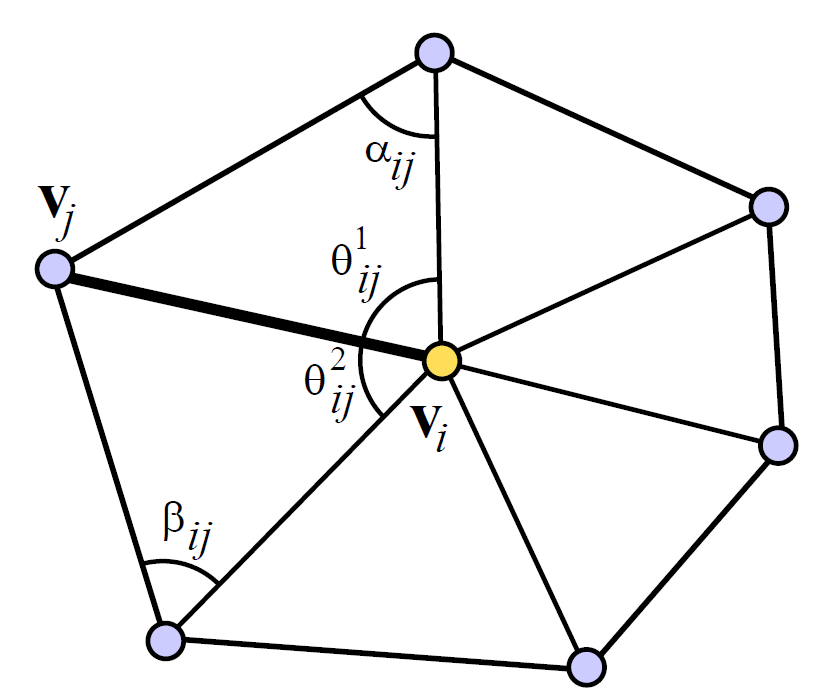
\includegraphics[width=0.5\linewidth]{cot_weight}
  \caption[Angles in cotangent weights]{Angles in cotangent weights (courtesy of \cite{Sorkine:EG:2005}).}
\label{fig:cotweights}
\end{figure}

To faithfully approximate smooth Laplacian on arbitrary meshes, we need to take
into account geometric information such as the distances between neighboring
vertices and the angles between contiguous edges. Such defined Laplacian is
called the \emph{geometric Laplacian}.

Constructing discrete Laplace-Beltrami operator on general meshes is not a trivial task.
In fact, it is impossible to make discrete Laplacian to simultaneously converge to smooth
Laplacian and be symmetric on general meshes~\cite{Rustamov:2007:LEF}. Many different
versions of geometric discrete Laplacian have been proposed
~\cite{pinkall1993computing, Desbrun1999, Xu:2004:GMP, Levy2006, Vallet2008, Belkin:2008:SCG}.
One of the most popular scheme was proposed by Meyer et al.~\cite{Meyer2003}.
It uses the cotangents of the two angles opposite to an edge to weight the edge,
and the area of the Voronoi cell size surrounding a vertex to weight the vertex.
Its action on vertex-based function $f$ on mesh $M$ is

\begin{equation}
\Delta f(v_i)=\frac{1}{a_i}\sum_{j\in N(i)}w_{ij}\frac{f(v_i)-f(v_j)}{d_i}.
\end{equation}

Here $a_i$ is the area of the Voronoi cells around vertex $v_i$, and the weights

\begin{equation}
w_{ij}:=\frac{\cot\alpha_{ij}+\cot\beta_{ij}}{2},
\end{equation}

where $\alpha_{ij}$ and $\beta_{ij}$ denote the two angles opposite to the edge $(v_i,v_j)$
(See Fig.~\ref{fig:cotweights}).

Let us define the area matrix $A=diag(a_i)$ and weight matrix $W$ as
\begin{equation*}
W(i,j)=\left\{
       \begin{array}{lc}
        \sum_{k\in N(i)}w_{ik}\quad & i=j \\
        -w_{ij}\quad & (v_i,v_j)\in E \\
        0\quad & \text{otherwise}
    \end{array}
\right.
\end{equation*}
The geometric Laplacian matrix then can be written as $L=A^{-1}W$.

Generally, such defined $L$ is not symmetric. However, we can rewrite the the 
equation $L\mathbf{\phi}=\lambda\mathbf{\phi}$ as the generalized eigenvalue 
problem

\begin{equation}
\label{eq:geneigen}
W\mathbf{\phi}=\lambda A\mathbf{\phi}.
\end{equation}

Since $W$ is symmetric and $A$ is symmetric positive-definite, the generalized 
eigenvectors $\mathbf{\phi_i}$ corresponding to different generalized eigenvalues 
$\lambda_i$ are orthogonal, and all of the generalized eigenvalues/eigenvectors 
are real. We should note that the orthogonality is with respect to the inner product
induced by $A$

\begin{equation}
\langle\mathbf{\phi_i},\mathbf{\phi_j}\rangle=\mathbf{\phi_i}^T A \mathbf{\phi_j}=0,\quad i\neq j.
\end{equation}

If the mesh vertices are evenly distributed, i.e., each vertex has the same Voronoi 
cell size, we can make $A=I$ by proper normalization. In this case, the $A$-inner 
product becomes the standard dot product ($I$-inner product). This is unfortunately 
not valid for general meshes whose vertices are not distributed uniformly over the 
surface area. We may adopt the symmetric version of mesh Laplacian $L_s = A^{-1/2}WA^{-1/2}$, 
which will give the same eigenvalues~\cite{Vallet2008}. The original eigenvectors can be 
obtained by $\mathbf{\phi_i}=W^{-1/2}\mathbf{\phi^s_i}$. However, this symmetrization is not 
preferable since solving the generalized eigenvalue problem is more stable than 
inverting $W$~\cite{Reuter:CG:2009}.

Let $\{\lambda_i\}_{i=0}^{N-1}$ be the set of generalized eigenvalues of
$\Delta_M=A^{-1}W$, and $\{\mathbf{\phi_i}\in\mathbb{R}^N\}$ their corresponding
eigenvectors. A square-integrable scalar function $\mathbf{f}$ defined on $V$ can 
be expanded as the linear combination of the eigenvectors

\begin{equation}
\mathbf{f}(p)=\sum_{k=0}^{N-1}\langle \mathbf{f},\mathbf{\phi_k}\rangle_A \mathbf{\phi_k}(p),
\end{equation}

where the inner-product is the $A$-induced scalar product

\begin{equation}
\langle \mathbf{f},\mathbf{g}\rangle_A = \mathbf{f}^T A\mathbf{g}=\sum_{i=0}^{N-1}a_i \mathbf{f}(i)\mathbf{g}(i).
\end{equation}

Unlike classic Fourier basis functions which are simply fixed sinusoids, the
manifold harmonic basis differ with the connectivity, geometry, and the type 
of Laplacian operator that is adopted~\cite{Zhang:2010:CGF}. As a result, the 
mesh Laplacian eigenvectors and eigenvalues actually encode substantial topological 
and geometric information and can help characterize the global shape property and 
reveal intrinsic structure of the original mesh. In addition, Laplace-Beltrami
operator is globally defined and is completely determined by the metric tensor, 
which is itself an isometry invariant. Hence, the Laplacian eigenvalues and eigenfunctions 
encode meaningful global intrinsic information about the shape and they are invariant 
under isometric deformations up to a change in sign~\cite{Rustamov:2007:LEF,Sun:2009:CGF}.
This lends to the popularity of spectral methods in the area of geometry processing 
and analysis. 

Directly employing the eigenstructures of mesh Laplacian, a great diversity of spectral
methods have been developed for shape modeling problems including compression~\cite{Karni2000},
segmentation~\cite{Liu2007}, deformation~\cite{Rong2008}, remeshing~\cite{dong2006spectral},
paramterization~\cite{Zhou2004}, shape indexing~\cite{Reuter:2006:CAD, Rustamov:2007:LEF},
and retrieval~\cite{Lavoue:2012}. We refer readers to \cite{Zhang:2010:CGF} for a more thorough
review of the theories and applications of mesh Laplacian spectra.

\section{Kernels and Spectral Graph Wavelets}

\subsection*{Kernel Functions}

The concept of manifold Fourier transform can be extended to the bivariate case to define kernel functions.
Suppose we have a bivariate kernel 
$\theta:\mathcal{M}\times\mathcal{M}\to\mathbb{R}$ which corresponds to a 
self-adjoint operator $\Theta$. The bivariate kernel $\theta$ can be expanded 
on the manifold Fourier basis

\begin{equation}
\theta(x,y)=\sum_{k=0}^\infty \hat{\theta}(k)\phi_k(x)\phi_k(y),
\end{equation}

where

\begin{equation}
\hat{\theta}(k)=\langle\langle\theta(x,y),\phi_k(x)\rangle,\phi_k(y)\rangle.
\end{equation}

$\hat{\theta}(k)$ can be deemed as the Fourier transform of the bivariate kernel 
with a slight abuse of language.

For example, the Laplace-Beltrami operator itself can be expanded as
\begin{equation}
\Delta_\mathcal{M}(x,y)=\sum_{i=0}^\infty \lambda_k\phi_k(x)\phi_k(y).
\end{equation}

Hence, its Fourier transform is $\widehat{\Delta_\mathcal{M}}(k)=\lambda_k$.

The kernel function $\theta(x,y)$ describes the relations between each pair of 
points on the manifold, and its diagonal $\theta(x,x)$ affords a
signature function for the characterization of individual points. 

One well known kernel function is the heat kernel $K(t,x,y)$, which is
the fundamental solution to the heat equation with appropriate boundary condition. 
Expanded on the manifold harmonic functions, the heat kernel with time parameter 
$t$ has the following expression:

\begin{equation}
K(t,x,y)=\sum_{k=0}^{\infty} e^(-\lambda_k t) \phi_k(x)\phi_k(y).
\end{equation}

On the mesh domain, the heat kernel affords a multi-scale, stable and intrinsic
characterization of the geometric shape~\cite{Sun:2009:CGF}, and have been 
the foundation for many shape analysis applications including shape matching~\cite{Ovsjanikov2010}
and shape retrieval~\cite{Bronstein2011}. 


\subsection*{Wavelets on Graphs}

Wavelet is a powerful analytical tool in signal processing. Intuitively speaking, 
a wavelet is just a wave-like pulse in time (or space). By scaling and translating
a single mother wavelet, we may obtain a family of wavelet functions that cover 
the entire domain in question. Similar to Fourier analysis in which a function $f$ 
can be decomposed into a series of component harmonics, in wavelet analysis $f$ 
can be expanded by a family of component wavelets. Nevertheless, there are some 
fundamental differences between the Fourier and wavelet analysis:

\begin{itemize}
\item In Fourier analysis, each component harmonic is globally defined in space/time. In wavelet analysis, the component wavelet are all locally defined at different locations.
\item In Fourier analysis, each component harmonic has an exclusive frequency. In wavelet analysis, we use multiple wavelets localized at different locations to represent the information of a single frequency. Generally, for large scale information (low frequency), we use fewer wavelets; whereas for small scale information (high frequency), we use more wavelets.
\item The component harmonics in Fourier analysis are all orthogonal to each other. In fact, the Fourier basis functions form an orthonormal basis of the space of square-integrable functions. This is not necessarily true for wavelet functions.
\end{itemize}

In a nutshell, wavelet functions can be simultaneously localized in both time/space and frequency domain,
in contrast to the Fourier transform in which the basis harmonic functions are all globally defined
in time/space. For signals whose primary information lies in localized singularities, such as edges
in images or step discontinuities in time series signals, wavelet transform affords a more compact
representations than a transform with global basis such as the Fourier transform.

There have been many efforts to introduce wavelet methods to the field of visual computing.
Representative applications include image segmentation \cite{Figueiredo:2005:CVPR},
image-based rendering \cite{Overbeck:2009:TOG}, volume rendering \cite{Lippert:1995},
scientific visualization \cite{Cracium:2005:TVCG}, spectral rendering \cite{Iehl:2000:CGF},
animation compression \cite{Payan:2007:CG}, etc.

Classical wavelets are constructed by translating and scaling a mother wavelet in Euclidean
space, however, transplanting wavelets to graphs (specifically, triangular meshes) is not
straightforward due in part to the fact that it is unclear how to apply the scaling operation
on a signal that is defined on the mesh vertices, so early studies using wavelet mostly
relied on the spherical parameterization~\cite{Werghi:2002,Liu:2007}.

One popular scheme to imitate scaling on meshed surfaces is achieved via explicit subdivision,
which iteratively refines the mesh geometry, and at the same time, also refines the functions
defined on the mesh. The constructed wavelets are biorthogonal and locally supported.
The subdivision wavelets rely on the subdivision connectivity of the mesh, which restricts the
application scope to data compression and level-of-detail rendering. The idea of subdivision
wavelets was first proposed by Schr\"{o}der and Sweldens \cite{Schroder:1995:SIGGRAPH}, in
which the lifting scheme was used to construct wavelets on sphere.
Lounsbery et al. \cite{Lounsbery:1997:TOG} studied MRA of wavelets constructed on surfaces
of arbitrary topology type. In \cite{Bertram:2000:vis}, Bertram et al. utilized bicubic
B-spline subdivision to construct wavelet transform that affords boundary curves and sharp
features. As a drawback, the subdivision wavelet
requires the meshes to have subdivision connectivity, where remeshing process is frequently
needed. To avoid remeshing, Valette and Prost \cite{Valette:2004:TVCG} extended the subdivision
wavelet for triangular meshes using irregular subdivision scheme that can be directly computed
on irregular meshes. On spherical domains, Haar wavelets \cite{Nielson:1997:vis,Bonneau:1999:vis}
were constructed over nested triangular grids generated by subdivision. Recently, the spherical
Haar wavelet basis was improved to the SOHO wavelet basis \cite{Lessig:2008:TOG} that is both
orthogonal and symmetric.

Another method to construct graph and mainfold wavelets is
through diffusion~\cite{Coifman2006, Hou2013}.
In sharp contrast to the aforementioned subdivision wavelets, the diffusion
wavelets adopt a bottom-up philosophy starting from the fine input data.
The \emph{Diffusion wavelets} ~\cite{Coifman2006} use a diffusion operator
and its powers to expand the nested subspaces, where scaling functions and
wavelet functions are obtained by orthogonalization and rank-revealing
compression. This diffusion-driven methodology naturally dilates the
functions associated with the underlying heat diffusion process, which solely
depends on manifold geometry. It allows flexible construction directly from data.
However, the constructed scaling and wavelet functions are not locally-supported,
which limits the functionality of space localization. In fact, it is impossible
to construct wavelets that are simultaneously fully orthogonal, locally supported,
and symmetric \cite{Lounsbery:1997:TOG}. As an improvement, the biorthogonal
diffusion wavelets (BDW) \cite{Maggioni:2005:SPIE} were introduced, relieving the
excessively-strict orthogonality property of scaling functions.
In \cite{Mahadevan2005}, diffusion wavelets were adopted to approximate
scalar-valued functions based on analyzing the structure and topology of the
state space. Rustamov \cite{Rustamov:2009:ICMS} studies the relation between
mesh editing and diffusion wavelets by introducing the generalized linear
editing (GLE). However, neither the DW nor the BDW have achieved localization
in both manifold and frequency domain.

In \cite{Hou2013}, an admissible diffusion wavelets (ADW) on meshed surfaces and point clouds is proposed.
The ADW are constructed in a bottom-up manner that starts from a local operator in a high frequency,
and dilates by its dyadic powers to low frequencies. By relieving the orthogonality and enforcing normalization,
the wavelets are locally-supported and admissible.

It is attractive to be able to define wavelet transform directly on 3D
shapes without the need of parameterization. Various schemes of
manifold wavelets have been proposed via different
approaches~\cite{Antoine2010189}. Diffusion wavelets, introduced by
Maggioni and Coifman~\cite{Coifman2006}, use diffusion as a
scaling tool to achieve multiscale analysis. Wavelet and scaling
functions are constructed by repeatedly applying a diffusion operator
$T$ on the graph or manifold space. After applying dyadic powers of
$T$ at each scale, a localized orthogonalization procedure is
performed to yield nested approximation spaces, and then wavelets are
produced by locally orthogonalizing vectors spanning the difference of
these approximation spaces. The derived diffusion wavelets are
orthogonal, compact, and multiscale in nature, and have been employed
in 3D mesh compression
in~\cite{mahadevan2007AdaMesCom3DComGraUsiMulManLea}.
In~\cite{gavish2010multiscale,ram2012redundant}, tree-based,
data-adaptive wavelet transforms are developed for high-dimensional
Euclidean data sets and weighted graphs, under the assumption that the
data have a rich geometrical structure that can be captured by a
hierarchical tree.

\subsection*{Spectral Graph Wavelets}

The primary reason that classical wavelet transforms cannot be directly adapted to graph or manifold is
that for a mother function $\psi(x)$ defined on a manifold,
there is no obvious definition for $\psi(sx)$. One approach to solve this problem is appealing to the Fourier domain,
with the help of aforementioned manifold harmonics. Although scaling cannot be explicitly expressed on manifold domain,
it can be easily defined on the frequency domain. The idea of spectral wavelet transform was introduced in \cite{Hammond2011}
on the graph domain, denoted as the Spectral Graph Wavelet Transform (SGWT). Here we extend the concept to general manifold,
denoted as the Spectral Graph Wavelet Transform (SGWT)

Given manifold $\mathcal{M}$ with appropriate boundary condition. Assume its Laplace-Beltrami operator $\Delta_\mathcal{M}$ has the eigen-decomposition $\{\lambda_k,\phi_k\}$. The eigenvectors $\{\phi_k\}$ form a complete and orthonormal basis of $L^2(\mathcal{M})$, commonly known as the manifold harmonics. The corresponding eigenvalues $\{\lambda_k\}$ satisfy
\begin{equation}
0=\lambda_0 < \lambda_1 \leq \lambda_2 \leq \cdots
\end{equation}

For any function $f$ defined on $\mathcal{M}$, its generalized Fourier transform $\hat{f}$ is defined as
\begin{equation}
\hat{f}(k)=\langle \phi_k, f \rangle=\sum_{k=0}^\infty \phi_k(x)f(x)
\end{equation}

And the inverse Fourier transform is
\begin{equation}
f(x)=\sum_{k=0}^\infty\hat{f}(k)\phi_k(x)
\end{equation}

The Parseval relations holds for the manifold harmonics transform
\begin{equation}
\label{eq:parseval}
\langle f,g\rangle=\langle\hat{f},\hat{g}\rangle
\end{equation}

\begin{figure}[!to]
\begin{center}
\includegraphics[width=\linewidth]{4_SGW}
\end{center}
\caption[Spectral graph wavelets on the wolf model.]{Spectral Graph Wavelets centered at one vertex on the wolf model.
  From left to right are wavelets from high frequency to low frequency with
  scale 1, 3 and 5.}
\label{SGW}
\end{figure}

We generate SGWT from a special wavelet operator that acts on functions defined on the manifold. Given a real-valued transfer function $g$, the wavelet operator $T_g$ is defined by how it modulate on $f:\mathcal{M}\to\mathbb{R}$ on Fourier domain
\begin{equation}
\widehat{T_g f}(k)=g(\lambda_k)\hat{f}(k)
\end{equation}

Employing the inverse Fourier transform, we obtain the spectral representation of $T_g f$
\begin{equation}
\label{eq:waveletop}
(T_g f)(\cdot)=\sum_{k=0}^\infty g(\lambda_k)\hat{f}(k)\phi_k(\cdot)
\end{equation}

To obtain spectral wavelets, we need localized and scaled versions of $T_g f$. The scaling is defined by dilating the transfer function as $g(t\lambda_k)$. The localization at point $x\in\mathcal{M}$ is realized by applying wavelet operators to unit impulse at $x$, represented by the Dirac delta function $\delta_x(\cdot)$

Since
\begin{equation}
\delta_x(\cdot)=\sum_{k=0}^\infty\phi_k(x)\phi_k(\cdot)
\end{equation}
We have the Fourier transform of $\delta_x$
\begin{equation}
\hat{\delta_x}(k)=\phi_k(x)
\end{equation}

Set $f=\delta_x$ in (\ref{eq:waveletop}), we have the spectral wavelet at scale $t$ and localized at point $x$
\begin{equation}
\psi_{t,x}(\cdot)=(T^t_g\delta_x)(\cdot)=\sum_{k=0}^\infty g(t\lambda_k)\phi_k(x)\phi_k(\cdot)
\end{equation}

The spectral wavelet can also be represented as a bivariate kernel
\begin{equation}
\Psi_t(x,y)=\psi_{t,x}(y)=\sum_{k=0}^\infty g(t\lambda_k)\phi_k(x)\phi_k(y)
\end{equation}

For a real-valued function $f$ defined on $\mathcal{M}$, the spectral wavelet transform is
\begin{equation}
\mathcal{W}^\psi_f(x,t)=\langle\psi_{x,t},f\rangle
\end{equation}

Applying the Parseval relation (\ref{eq:parseval}), we obtain the spectral representation of continuous spectral wavelet transform
\begin{equation}
\mathcal{W}^\psi_f(x,t)=\langle\hat{\psi_{x,t}},\hat{f}\rangle=\sum_{k=0}^\infty\hat{\psi_{x,t}}(k)\hat{f}(k)=\sum_{k=0}^\infty g(t\lambda_k)\hat{f}(k)\phi_k(x)
\end{equation}

If seen as a function of $x$, the Fourier transform of the above spectral wavelet transform is
\begin{equation}
\widehat{\mathcal{W}^\psi_f}(k)=g(t\lambda_k)\hat{f}(k)
\end{equation}

Similar to classical wavelet transform, the spectral wavelet transform is invertible only if the transfer function $g$ satisfies the admissibility condition
\begin{equation}
C_\psi=\int_0^\infty\frac{g^2(a)}{a}da<\infty
\end{equation}
and the zero-mean condition $g(0)=0$.

%Then we consider the summation of wavelets $\psi_{t,x}$ multiplied by corresponding wavelet coefficient $\mathcal{W}^\psi_f(t,x)$, subject to a non-constant weight $dt/t$
%\begin{align*}
%  & \sum_{x\in\mathcal{M}}\int_0^\infty\frac{\mathcal{W}^\psi_f(x,t)\psi_{x,t}(y)}{t}dt \\
%= & \int_0^\infty\frac{dt}{t}\sum_{x\in\mathcal{M}}\mathcal{W}^\psi_f(x,t)\psi_{y,t}(x) \\
%= & \int_0^\infty\frac{dt}{t}\sum_{k=0}^\infty\hat{\mathcal{W}}^\psi_f(k)\hat{\psi}_{y,t}(k) \\
%= & \int_0^\infty\frac{dt}{t}\sum_{k=0}^\infty(g(\lambda_k t)\hat{f}(k))(g(\lambda_k t)\phi_k(y)) \\
%= & \sum_{k=0}^\infty(\int_0^\infty\frac{|g(\lambda_k t)|^2 dt}{t})\hat{f}(k)\phi_k(y) \\
%= & (\int_0^\infty\frac{|g(a)|^2da}{a})\sum_{k=1}^\infty\hat{f}(k)\phi_k(y) \\
%= & C_\psi(f(y)-\hat{f}(0)\phi_0(y))
%\end{align*}

%This yields the formula of inverse continuous spectral wavelet transform
%\begin{equation}
%f(y)=\frac{1}{C_\psi}\int_0^\infty\frac{\mathcal{W}_f^\psi(x,t)\psi_{x,t}(y)}{t}dt+\hat{f}(0)\phi_0(y)
%\end{equation}

\begin{figure}
  \centering
  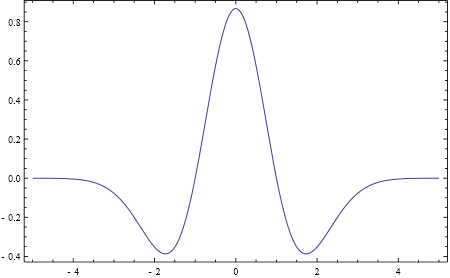
\includegraphics[width=0.5\linewidth]{1DMexicanHat}\\
  \caption{1D Mexican-hat Wavelet}
  \label{fg:1DMexicanHat}
\end{figure}

\begin{figure}
  \centering
  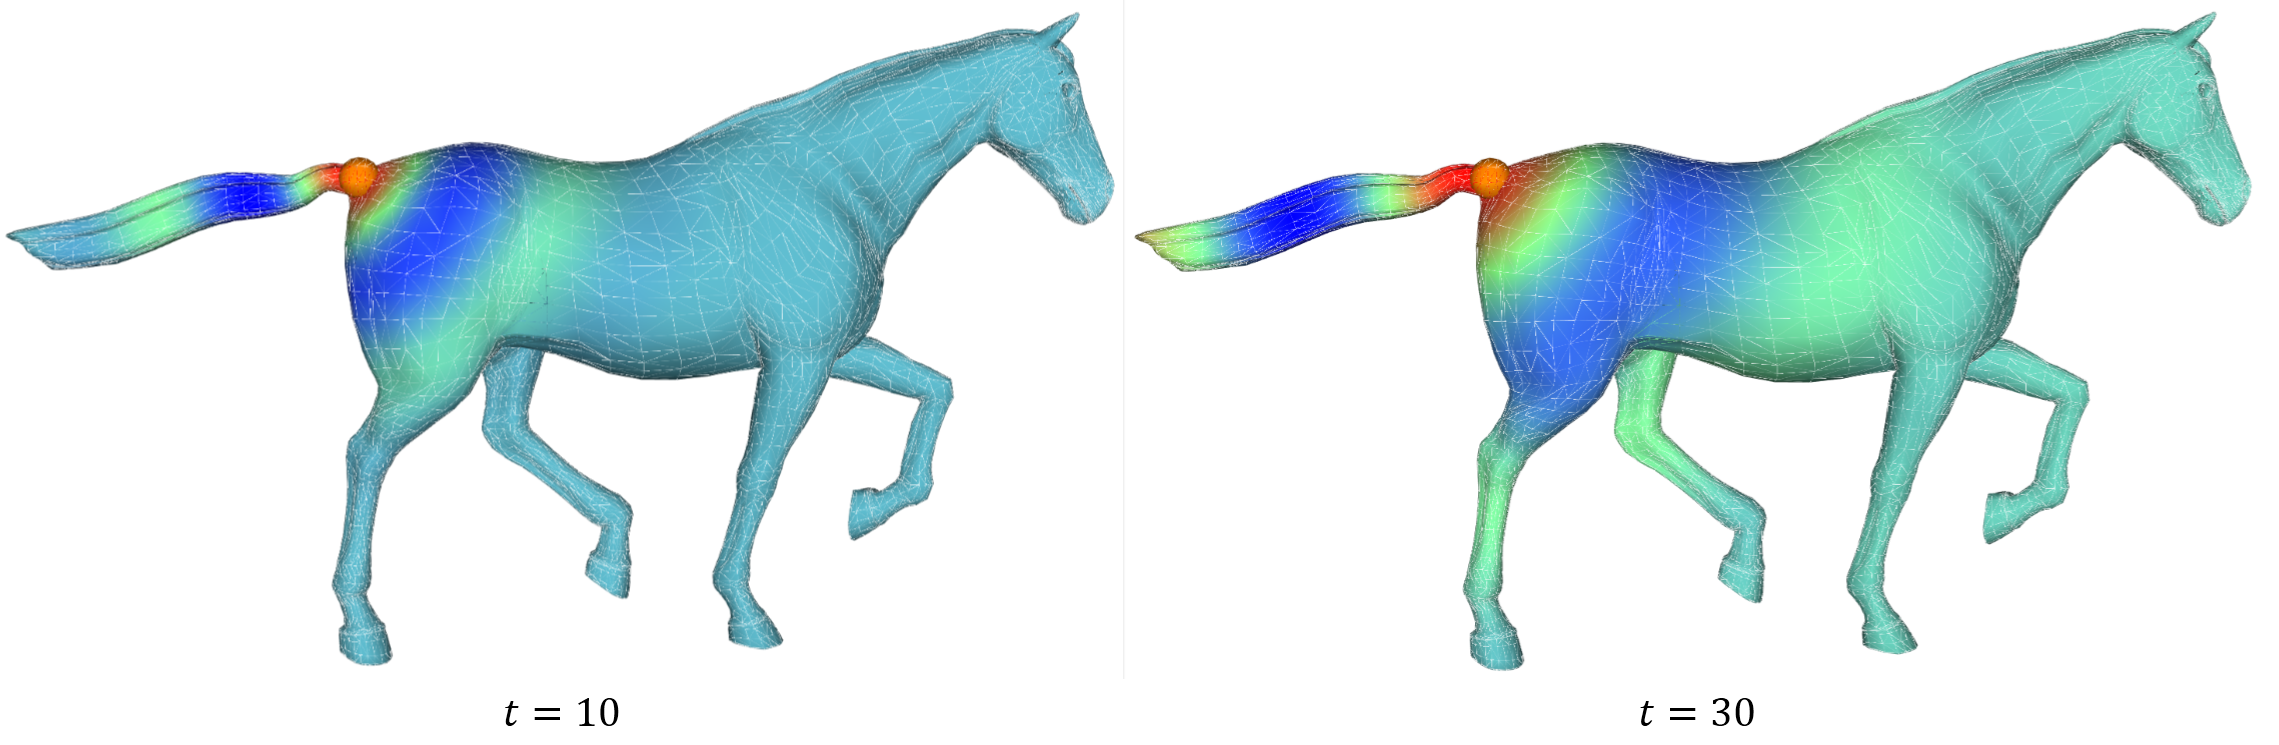
\includegraphics[width=\linewidth]{MexicanHatWavelet}\\
  \caption[Color plots of the spectral Mexican-hat wavelets.]
  {Color plots of the spectral Mexican-hat wavelet with scales of 10 and 30. The reference point is denoted by the orange ball. We can easily spot the function values oscillate around the reference point. When t is larger, the period of oscillation also increases.}
  \label{fg:MexicanHatWavelet}
\end{figure}

\begin{figure}
  \centering
  \includegraphics[width=0.8\linewidth]{WaveletFrequency}\\
  \caption[Transfer function of the Mexican-hat wavelet.]
  {The Mexican-hat wavelet transfer function in the frequency domain. }\label{fg:WaveletFrequency}
\end{figure}

In classical wavelets defined on real line, the space localization is apparent. If the mother wavelet $\psi(x)$ is localized in the interval $[-\epsilon,\epsilon]$, then the wavelet $\psi_{a,b}(x)$ will be localized with $[b-a\epsilon,b+a\epsilon]$. in the limit as $b\to 0$, $\psi_{a,b}(x)\to 0$ for $x\neq b$.

For spectral wavelets, the localization property is less straightforward since the scaling is defined implicitly in the Fourier domain. For $g$ sufficiently regular, the normalized spectral wavelet $\psi_{t,x}/\|\psi_{t,x}\|$ will vanish on vertices sufficiently far from $x$ in the limit of fine scales, i.e. as $t\to 0$. We should expect $\psi_{t,x}(y)$ to be small if $x$ and $y$ are separated and $t$ is small.

If two transfer functions $g$ and $g'$ are close to each other, then the derived spectral wavelets should be close to each other in the manifold domain.

As an example, we consider the Mexican hat wavelet. In 1D Euclidean space, the Mexican hat wavelet is defined as
\begin{equation}
\psi(t)=\frac{2}{\sqrt{3\sigma}\pi^{\frac{1}{4}}}(1-\frac{t^2}{\sigma^2})e^{\frac{-t^2}{2\sigma^2}}.
\end{equation}
Its graph is shown in Fig.~\ref{fg:1DMexicanHat}, which exhibits clear localization in space. In manifold space, we may analogously define the spectral Mexican hat wavelet as
\begin{equation}
\psi_{t,x}(\cdot)=\sum_{k=0}^\infty t^2\lambda_k^2 e^{-t^2\lambda_k^2}\phi_k(x)\phi_k(\cdot),
\end{equation}
with the transfer function $g(t\lambda)=t^2\lambda^2 e^{-t^2\lambda^2}$.

Fig.~\ref{fg:MexicanHatWavelet} visualizes the value of the wavelet functions over the surface, with the scale $t=10$ and $t=30$. Fig.~\ref{fg:WaveletFrequency} shows the Fourier transform of the wavelet functions in frequency domain. It is easy to see that

\begin{itemize}
\item The spectral wavelet function is localized both in manifold and frequency domain.
\item On manifold, the values of the spectral wavelet functions attenuate and oscillate as the distance from the reference point increases.
\item For a larger scale, the Mexican hat wavelet has a wider windows in space, but a narrower window in frequency.
\end{itemize}

By construction, the spectral wavelets $\psi_{t,x}$ are all orthogonal to the the null eigenvector $\phi_0$,
and nearly orthogonal to $\phi_l$ for $\lambda_l$ near zero \cite{Hammond2011}.

Spectral scaling functions are determined by a single real valued function $h:\mathbb{R}^+\to\mathbb{R}$,
which acts as a low-pass filter and satisfies $h(0)>0$ and $\lim_{x\to\infty}h(x)\to 0$.
Introducing the scaling functions helps ensure stable recovery of the original signal $f$ from the wavelet
coefficients when the scale parameter $t$ is sampled at discrete values ${t_j}$.
Stable recovery will be assured if $G(\lambda)=h(\lambda)^2+\sum_{j=1}^J g(t_j\lambda)^2$ is
bounded away from zero. The design of the scaling function generator $h$ is uncoupled from the choice $g$.

The spectral wavelets depend on the continuous scale parameter $t$. For practical computation,
$t$ must be sampled at a finite number of scales $\{t_j\}_{j=1}^J$, which generates
$NJ$ wavelets $\psi_{t_j,n}$ along with $N$ scaling functions $s_n$. It can be proven~\cite{Hammond2011}
that the set $\Gamma=\{\phi_n,n=0,\ldots,N-1\}\cup\{\psi_{t_j,n},j=1,\ldots,J,n=1,\ldots,N\}$
form a frame with bounds
\begin{equation*}
A=\min_{\lambda\in[0,\lambda_{N-1}]}G(\lambda)
\end{equation*}
and
\begin{equation*}
B=\max_{\lambda\in[0,\lambda_{N-1}]}G(\lambda),
\end{equation*}
where $G(\lambda)=h^2(\lambda)+\sum_j g(t_j\lambda)^2$. That is to say, for all $f$ defined on the manifold, the following inequality holds
\begin{equation}
A\|f\|^2\leq\sum_k|\langle f,\Gamma_k\rangle|^2\leq B\|f\|^2,
\end{equation}
where $\Gamma=\{\Gamma_k\}$.

The spectral wavelet transform is an overcomplete transform, mapping
an input vector $f$ of size $N$ to $N(J+1)$ coefficients $c=Wf$.
Given a set of coefficients $c$, the synthesis/reconstruction of $f$ can be given by solving the matrix equation
\begin{equation}
(W^*W)f=W^*c.
\end{equation}

Because of its attractive and powerful properties such as spatial localization, 
multiscale, and geometry awareness, SGW has already been adopted as a descriptor 
for a handful of shape analysis applications. Kim et al.~\cite{Kim:2012,Kim:2014}
introduced a wavelet-based multi-scale descriptor for the analysis of
cortical surface signals using the SGWT and Li et al.~\cite{Li:2013}
proposed a SGWT-based descriptor and utilized the intrinsic spatial
pyramid matching (ISPM) for global shape retrieval. Though these
researches discover the potentials of SGWs, they all concentrate on
global shape analysis based on point signatures, ignoring the SGWs'
power in integrating the local-to-global geometrical and topological information.

\section{Sparse Representation Modeling}

In recent years, sparse modeling techniques have become
increasingly popular in various fields of signal processing and
analysis, especially in image processing and computer vision. Its
widespread applications include data compression, signal denoising,
pattern recognition, etc.

The fundamental idea of sparse modeling is to decompose or approximate the
signal in question as the linear combination of a very small subset of vectors
selected from a large number of candidate elementary vectors. These candidate
elementary vectors, also called \emph{atoms}, constitute a set called the
\emph{dictionary}. With a given dictionary, the signal is encoded by the
coefficients w.r.t. the selected atoms and can be easily reconstructed. The
rationale of sparse modeling is that most meaningful high-dimensional signals probably
have some intrinsic structures or patterns, which can be exploited for
efficient representation in a subspace of much lower dimension. Because of
the versatility of the input signals, it is often desirable for dictionaries to
be redundant or overcomplete, allowing greater freedom and flexibility in
design to accommodate a sparse set of atoms that can better capture
an input signal's intrinsic characteristics.

\subsection{Sparse Modeling Problems}

Consider signal $\mathbf{b}\in\mathbb{R}^n$ and dictionary matrix
$\mathbf{D}\in\mathbb{R}^{n\times m}$ with $n<m$. If the dictionary constitutes an
overcomplete basis of $\mathbb{R}^n$, the linear systems of
equations $A\mathbf{x}=\mathbf{b}$ is underdetermined and has infinite solutions.

To make the solution $\mathbf{x}$ unique, we could introduce an objective function
$J(\mathbf{x})$ to govern the desired properties of the solution vector $\mathbf{x}$.
The general optimization problem subject to linear equality constraints is as follows:

\begin{equation}
\label{eq:constrained-inverse}
\min_\mathbf{x} J(\mathbf{x}) \quad \mathrm{subject\,to} \quad \mathbf{b}=\mathbf{D}\mathbf{x}.
\end{equation}

Alternatively, the objective function can be used as a regularization term, giving rise to
the following regularized least square problem:

\begin{equation}
\label{eq:regularized-ls}
\min_\mathbf{x} \|\mathbf{b}-\mathbf{D}\mathbf{x}\|_2^2 + \lambda J(\mathbf{x}).
\end{equation}

The regularization term can be viewed as imposing certain priors distributions on
the solution $\mathbf{x}$. Comparing with Eq.~\ref{eq:constrained-inverse}, regularization
allows users to control the tradeoff between the reconstruction fidelity and the
desired property (e.g., smoothness) of the solution and avoids overfitting.

Eq.~\ref{eq:constrained-inverse} and Eq.~\ref{eq:regularized-ls} are commonly encountered in different
areas, including signal processing, machine learning, and statistics. One common choice for $J(\mathbf{x})$
is the function of squared $l_2$-norm $\|\mathbf{x}\|_2^2$, which aims to minimize the ``energy'', or Euclidean
norm of the solution vector. Eq.~\ref{eq:constrained-inverse} then has the closed-form

\begin{equation}
\hat{\mathbf{x}}=\mathbf{D}^T(\mathbf{D}\mathbf{D}^T)^{-1}\mathbf{b}=\mathbf{D}^{+}\mathbf{b},
\end{equation}
where $\mathbf{D}^{+}=\mathbf{D}^T(\mathbf{D}\mathbf{D}^T)^{-1}$ is the pseudo-inverse
of $\mathbf{D}$. Let $J(\mathbf{x})=\mathbf{\Gamma}\mathbf{x}$, where $\mathbf{\Gamma}\in\mathbb{R}^{m\times m}$,
Eq.~\ref{eq:regularized-ls} then becomes the famous Tikhonov regularization~\cite{Golub1999}, which has the
explicit solution
\begin{equation}
\hat{\mathbf{x}} = (\mathbf{D}\mathbf{D}^T + \lambda \mathbf{\Gamma}\mathbf{\Gamma}^T)^{+}\mathbf{D}^T\mathbf{b}.
\end{equation}

Due to its computational simplicity, the $l_2$ norm is commonly used as the or penalty term. However, for
many applications, minimizing the total energy of solutions is not very meaningful.

If we know that the signal $\mathbf{b}$ has a very sparse coefficient representation $\mathbf{x'}$ with respect
to $\mathbf{D}$, i.e., $ \mathbf{b} \approx \mathbf{D}\mathbf{x'}, \|\mathbf{x'}\|_0 \ll m$,
then we can specify $J(\mathbf{x})$ such that the objective to minimize the number of non-zero coefficients
in solution $\mathbf{x}$. The resultant optimization problem is called sparse decomposition and can be
formulated as follows:

\begin{equation}
\label{eq:sparse-decompose}
\min_\mathbf{x} \|\mathbf{x}\|_0 \quad \mathrm{subject\,to} \quad \mathbf{b}=\mathbf{D}\mathbf{x}.
\end{equation}

Here $\|\mathbf{x}\|_0$ denotes the pseudo norm of $\mathbf{x}$ which counts the number
of non-zero elements in $\mathbf{x}$.

For real life signals, exact sparsity w.r.t. a fixed dictionary is elusive; instead, natural
signals tend to be \emph{compressible}, meaning that the representation coefficients decay rapidly
when sorted in order of decreasing magnitude. Hence, a more practical formulation is to allow a bounded
error of the sparsely reconstructed signal $\mathbf{D}\mathbf{x}$, giving rise to the best
subset selection problem:
\begin{equation}
\label{eq:sparse-approx}
\min_\mathbf{x} \|\mathbf{x}\|_0 \quad \mathrm{subject\,to} \quad \|\mathbf{b}-\mathbf{D}\mathbf{x}\|_2^2<\epsilon.
\end{equation}
or written as a regularization problem,
\begin{equation}
\label{eq:regularized-sparse-approx}
\min_\mathbf{x}  \|\mathbf{b}-\mathbf{D}\mathbf{x}\|_2^2 + \lambda \|\mathbf{x}\|_0
\end{equation}

Clearly, the approximation quality and the sparsity of the coefficient vector depend both on the signal itself
and the dictionary $\mathbf{D}$. We can expect more concise and accurate coefficient representations if the atoms
in $\mathbf{D}$ can better capture properties of concerned signal. Take the 2D image domain as example. The global
Fourier basis vectors are suitable for representing global signal trends, while wavelets, with its local support,
can better represent isotropic features of different scales. To efficiently encode anisotropic image feature
such as lines and curves, various extensions to wavelets have been proposed
including contourlet~\cite{Do2005}, ridgelets~\cite{Emmanuel1999}, curvelets~\cite{Candes1999}, etc. By incorporating
new design parameters such as directions, these new shape basis afford more effective characterization of images
dominated with different features.

\subsection{Computational Methods}
The $l_0$ optimization problems (Eq.~\ref{eq:sparse-decompose} and Eq.~\ref{eq:sparse-approx}) are NP-hard,
so searching through all possible support sets by brute force is intractable except for problems of very small
sizes. A variety of methods have been developed for finding near-optimal solution to $l_0$ optimization, and
the most important two classes are \emph{greedy pursuit} and \emph{convex relaxation}~\cite{Tropp2010}.

\subsubsection*{Greedy Pursuit Methods}
One of the most commonly-used approaches to sparse approximation is
the greedy pursuit method. The central idea is to iteratively refine a
sparse solution in a greedy manner. More specifically, in each
iteration one or more atoms of the dictionary are chosen
and the corresponding coefficients are modified
such that the greatest improvement in approximation quality can be achieved.
Representative greedy pursuit algorithms include matching pursuit
(MP)~\cite{Mallat1993}, orthogonal matching pursuit
(OMP)~\cite{Pati1993}, and simultaneous orthogonal matching pursuit (S-OMP)~\cite{Tropp2006a}.
The latter is suitable for solving the simultaneous sparse approximation problem where
the input signal have multiple correlated channels and the same subset of atoms is to be used
for every channel.


The basic idea of greedy pursuit methods is to iterative refine the estimation of the coefficient vector
$\mathbf{x}$. In each step, one or several coefficients are modified to yield biggest possible improvement
in approximating the signal. The simplest greedy pursuit algorithm is \emph{matching pursuit (MP)}~\cite{Mallat1993},
described as follows
\begin{enumerate}
\item Set the index set $\Omega=\emptyset$, the residual $\mathbf{r_0} = \mathbf{b}$, and the counter $k=1$.
\item Find an index $n_k$ such that atom $\mathbf{\alpha}_{n_k}$ is most correlated with the residual
\begin{equation*}
n_k = \argmax_n |\langle \mathbf{r}_{k-1},\mathbf{\alpha}_{n} \rangle|,
\end{equation*}
and add $n_k$ to $\Omega$. The coefficient corresponding to $\mathbf{\alpha}_{n_k}$ is denoted as $x_{n_k}$.

\item Update the residual $\mathbf{r}_k = \mathbf{r}_{k-1} - x_{n_k} \mathbf{\alpha}_{n_k}$.
\item Increment $k$. Repeat (2)-(4) until stopping criterion is met.
\end{enumerate}

The possible stopping criteria can be that a fixed number of atoms have been selected, the magnitude of residual is
smaller than a threshold, or no remaining atoms have strong correlation with the residual.

A much improved version of MP is the algorithm known as \emph{orthogonal matching pursuit (OMP)}~\cite{Pati1993}.
The major difference with MP is an additional step of coefficients update. After a new index (that is most strongly
correlated with the residual) is identified and added to the index set $\Omega$,
the coefficients calculated in previous steps are replaced with new coefficients which approximate the original signal
in the least square sense. Contemporary greedy pursuit methods have more sophisticated mechanism for selecting and
pruning the set of active atoms, including the stagewise orthogonal matching pursuit (StOMP)
~\cite{Donoho2012}, regularized orthogonal matching pursuit~\cite{Tropp2007}, and compressive sampling matching
pursuit (CoSaMP)~\cite{Needell2009}. Apart from greedy selection, another method to achieve greedy pursuit is
iterative thresholding, or \emph{shrinkage} ~\cite{Daubechies2004, Blumensath2009}. The basic idea is to
iterative updating the coefficients with thresholding applied in each step to enforce sparsity.

Theoretically, it has been proved that greedy pursuit methods can produce near-optimal sparse approximations
if the dictionary is sufficiently incoherent~\cite{Tropp2004}. If the dictionary is sufficient random and the
signal is sparse enough, simple pursuit methods can provably recover the sparse representation with high probability~\cite{Tropp2007}.


\subsubsection*{Convex Relaxation Methods}
Another approach to sparse approximation problems is to replace the highly discontinuous $l_0$ norm
with $l_1$ norm, yielding $l_1$ optimization problems which are convex and tractable.
This convex relaxation is generally reasonable, as it has been proved that for most large underdetermined system,
$l_1$ and $l_0$ minimization will produce the same unique solution, provided the signal is sufficiently
sparse~\cite{donoho2006most}.

The two most common $l_1$ optimization problems are \emph{basis pursuit}
\begin{equation}
\label{eq:basis-pursuit}
\min_\mathbf{x} \|\mathbf{x}\|_1 \quad \mathrm{subject\,to} \quad \mathbf{b}=\mathbf{D}\mathbf{x},
\end{equation}
and \emph{basis pursuit denoising (BPDN)}
\begin{equation}
\label{eq:bpdn}
\min_\mathbf{x} \frac{1}{2}\|\mathbf{b}-\mathbf{D}\mathbf{x}\|_2^2 + \lambda \|\mathbf{x}\|_1,
\end{equation}
where the parameter $\lambda$ is a regularization parameter which governs the sparsity of the solution.

Practical methods for solving $l_1$ optimization include \emph{interior point methods}~\cite{Chen2001,Candes2005,Kim2007},
iteratively reweighted least squares (IRLS) algorithm~\cite{Rao2003,Chartrand2008,Daubechies2010}, and stepwise algorithms
~\cite{Osborne2000, Plumbley2005, Efron2004}. We refer readers to \cite{Bruckstein2009} and \cite{Tropp2010} for more detailed review of the algorithms for sparse solution of underdetermined linear system.


\subsection{Applications}

Sparsity-drive signal processing have numerous applications, and the following
are the most commonly encountered.

\begin{itemize}

\item \textbf{Analysis.} Given signal $\mathbf{y}$ which is generated from a sparse
coefficient vector $\mathbf{x}_0$ with respect to dictionary $\mathbf{A}$, i.e.,
$\mathbf{y}=\mathbf{A}\mathbf{x}_0$, we can compute a sparse approximation of
$\mathbf{y}$ by solving Eq.~\ref{eq:regularized-sparse-approx}. Under certain
incoherent and sparsity conditions, the sparse solution $\mathbf{x}$ can well
recover the true underlying vector $\mathbf{x}_0$.

\item \textbf{Compression.} With greedy pursuit algorithms such as OMP, a
 nonlinear approximation of the original signal can be easily
 computed, yielding a compressive coefficient representation that can best
 approximate the original signal.

\item \textbf{Denoising.} Suppose the observation of the original sparse
signal $\mathbf{y}=\mathbf{A}\mathbf{x}_0$ is the noisy version $\mathbf{\tilde{y}}=\mathbf{y}+\mathbf{v}$.
When $\mathbf{x}_0$ is sufficiently sparse, it can often be reliably recovered
by solving the sparse approximation problem, which subsequently yields a
denoised signal.

\item \textbf{Compressed sensing.} Let $P\in\mathbb{R}^{j\times n}$ be a
measurement matrix of the original sparse signal
$\mathbf{y}=\mathbf{A}\mathbf{x}, \mathbf{y}\in\mathbb{R}^n$
and $j < n$. Given measure $\mathbf{c}=P\mathbf{y}$, the sparse coefficient vector
$\mathbf{x}$ can be recovered by solving
\begin{equation}
\min_\mathbf{x} \|\mathbf{x}\|_0 \quad \mathrm{subject\,to} \quad \|\mathbf{c}-\mathbf{P}\mathbf{A}\mathbf{x}\|_2 \leq \epsilon,
\end{equation}
as long as the original signal is sufficiently sparse and the sensing matrix $\mathbf{P}$ conforms to restricted isometry property.
The original signal then can be recovered from the coefficient representation.

\item \textbf{Source separation.} Suppose the observed signal $\mathbf{y}$ is the superposition of
two different sub-signals $\mathbf{y_1}$, $\mathbf{y_2}$, which are sparsely generated with dictionaries
$\mathbf{A}_1$ and $\mathbf{A}_2$, respectively. The sparse coefficient vectors of the two sub-signals
can be estimated by solving the following optimization problem
\begin{equation}
\hat{\mathbf{x}}_1,\hat{\mathbf{x}}_2 = \min_{\mathbf{x}_1,\mathbf{x}_2} \|\mathbf{x}_1\|_0 + \|\mathbf{x}_2\|_0 \quad \mathrm{s.t.} \quad \|\mathbf{y}-\mathbf{A_1 x_1} - \mathbf{A_2 x_2}\|_2^2 \leq \epsilon_1^2 + \epsilon_2^2,
\end{equation}
and the separate sub-signals can be reconstructed as $\hat{\mathbf{y}}_1=\mathbf{A}_1\hat{\mathbf{x}}_1$ and $\hat{\mathbf{y}}_2=\mathbf{A}_2\hat{\mathbf{x}}_2$.

\end{itemize}


